\documentclass[12pt]{article}
%\usepackage[utf8]{inputenc}
%\documentclass[UTF8]{ctexart}
%\usepackage[UTF8, heading = false, scheme = plain]{ctex}
\usepackage{geometry}
%geometry{a4paper,scale=0.9}
\geometry{a4paper,left=1cm,right=1cm,top=1cm,bottom=2cm}
\usepackage{amsfonts}
\usepackage{color}
\usepackage{url}
%\usepackage{biblatex}
\usepackage{amsmath}
\usepackage{amssymb}
\usepackage{latexsym}
\usepackage{cite}
%\addbibresource{ref.bib}
%\bibliography{ref.bib}
\usepackage{caption}
\usepackage{graphicx, subfig}
\usepackage{float}
%\usepackage[fontset=ubuntu]{ctex}
%\usepackage{fontspec}
\usepackage{xeCJK}
%\usepackage[colorlinks,
%anchorcolor=black,
%citecolor=black]{hyperref}
%\setmainfont{SimSun}
\usepackage[section]{placeins}
\usepackage{enumitem}
\usepackage{framed}
\usepackage[framemethod=TikZ]{mdframed}
\usepackage{indentfirst}
\usepackage{setspace}%使用间距宏包
\linespread{1.5}
%\title{预备知识}
%\author{leolinuxer }
%\date{June 2020}

\title{线性代数与微积分}
\author{leolinuxer}
%\date{June 2020}

\begin{document}
\maketitle

\section{矩阵求导相关\cite{Brief_Introduction_Of_Derivative_Of_Matrix}}
矩阵求导的几种组合形式:
\begin{figure}[H]
\centering
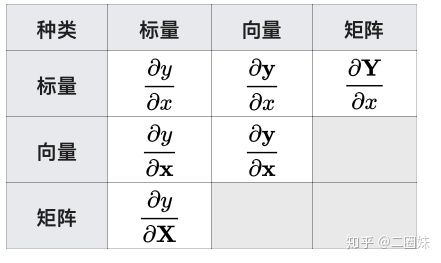
\includegraphics[width=.5\textwidth]{fig/DerivativeOfMatrix_1.jpg}
\end{figure}

\subsection{向量对标量求导 (Vector-by-scalar)}
向量 $\mathbf{y} = [y_1, y_2, \cdots, y_n]^T$ ,对标量 $x$求导,一般写为:
$$
\frac{\partial \mathbf{y}}{\partial x} = \begin{bmatrix}
\frac{\partial y_1}{\partial x} \\
\frac{\partial y_2}{\partial x} \\
\vdots \\
\frac{\partial y_n}{\partial x}
\end{bmatrix}
$$

\subsection{标量对向量求导(Scalar-by-vector)}
标量 $y$ 对 向量 $\mathbf{x} = [x_1, x_2, \cdots, x_n]^T$ 求导写作:
$$
\frac{\partial y}{\partial \mathbf{x}} = [\frac{\partial y}{\partial x_1}, 
\frac{\partial y}{\partial x_2},
\cdots,
\frac{\partial y}{\partial x_n}
]
$$

这里可能会让人疑惑,为什么上面是列向量而这里则是行向量。

这是矩阵求导可能会比较麻烦的地方,可能有不同的布局方式:
\begin{itemize}
    \item 分子布局(Numerator Layout):分子不变,分母转置
    \item 分母布局(Denominator Layout):分母不变,分子转置
\end{itemize}

当然还有混合布局。

用分子布局因为 wikipedia 里就是这样做的,而且有些只能有分子布局表示。

\subsection{向量对向量求导(Vector-by-vector)}
向量 $\mathbf{y} = [y_1, y_2, \cdots, y_m]^T$对向量 $\mathbf{x} = [x_1, x_2, \cdots, x_n]^T$求导,同样分子布局:
$$
\frac{\partial \mathbf{y}}{\partial \mathbf{x}} = 
\begin{bmatrix}
    \frac{\partial y_1}{\partial x_1} &
    \frac{\partial y_1}{\partial x_2} & 
    \cdots &
    \frac{\partial y_1}{\partial x_n} \\
    \frac{\partial y_2}{\partial x_1} &
    \frac{\partial y_2}{\partial x_2} & 
    \cdots &
    \frac{\partial y_2}{\partial x_n} \\
    \vdots & \vdots &  & \vdots \\
    \frac{\partial y_m}{\partial x_1} &
    \frac{\partial y_m}{\partial x_2} & 
    \cdots &
    \frac{\partial y_m}{\partial x_n} \\
\end{bmatrix}
$$

正好是雅克比矩阵:
$$
\mathbf{J} = [
\frac{\partial \mathbf{f}}{\partial x_1}, 
\frac{\partial \mathbf{f}}{\partial x_2},
\cdots,
\frac{\partial \mathbf{f}}{\partial x_n}] = 
\begin{bmatrix}
    \frac{f_1}{\partial x_1} &
    \cdots &
    \frac{f_1}{\partial x_n} \\
    \vdots &  & \vdots \\
    \frac{f_m}{\partial x_1} &
    \cdots &
    \frac{f_m}{\partial x_n}
\end{bmatrix}
$$

这是使用分子布局的好处,否则就是雅克比的转置了。

这样的好处是写下这个式子也很自然:
$$
\mathbf{f}(\mathbf{x}) - \mathbf{f}(\mathbf{p}) = \mathbf{J}_f(\mathbf{p})(\mathbf{x}-\mathbf{p}) + o(||\mathbf{x} - \mathbf{p}||) \quad (as \quad \mathbf{x} \rightarrow \mathbf{p})
$$

\subsection{矩阵对标量求导 (Matrix-by-scalar)
}
$$
\frac{\mathbf{Y}}{x} = 
\begin{bmatrix}
    \frac{\partial y_{11}}{\partial x} &
    \frac{\partial y_{12}}{\partial x} & 
    \cdots &
    \frac{\partial y_{1n}}{\partial x} \\
    \frac{\partial y_{21}}{\partial x} &
    \frac{\partial y_{22}}{\partial x} & 
    \cdots &
    \frac{\partial y_{2m}}{\partial x} \\
    \vdots & \vdots &   & \vdots \\
    \frac{\partial y_{m1}}{\partial x} &
    \frac{\partial y_{m2}}{\partial x} & 
    \cdots &
    \frac{\partial y_{mn}}{\partial x} \\
\end{bmatrix}
$$

\subsection{标量对矩阵求导(Scalar-by-matrix)}
$$
\frac{y}{\mathbf{X}} = 
\begin{bmatrix}
    \frac{\partial y}{\partial x_{11}} &
    \frac{\partial y}{\partial x_{12}} & 
    \cdots &
    \frac{\partial y}{\partial x_{1q}} \\
    \frac{\partial y}{\partial x_{21}} &
    \frac{\partial y}{\partial x_{22}} & 
    \cdots &
    \frac{\partial y}{\partial x_{2q}} \\
    \vdots & \vdots &  & \vdots \\
    \frac{\partial y}{\partial x_{p1}} &
    \frac{\partial y}{\partial x_{p2}} & 
    \cdots &
    \frac{\partial y}{\partial x_{pq}} \\
\end{bmatrix}
$$

\begin{framed}  
%\verb|\documentstyle[ifthen,12pt,titlepage]{article}|
矩阵求导本质上还是对单个变量求导,来看一个例子,比如:
$$
\frac{\partial (\mathbf{A}\mathbf{x})}{\partial \mathbf{x}}
$$

先来计算$\mathbf{A}\mathbf{x}$
$$
\mathbf{A}\mathbf{x} = \begin{bmatrix}
    A_{11} & \cdots & A_{1n} \\
    \vdots &        & \vdots \\
    A_{m1} & \cdots & A_{mn} \\
\end{bmatrix}
\begin{bmatrix}
   x_1 \\ \vdots x_n
\end{bmatrix}
= 
\begin{bmatrix}
A_{11}x_1 + A_{12}x_2 + \cdots + A_{1n}x_n \\
\vdots \\
A_{m1}x_1 + A_{m2}x_2 + \cdots + A_{mn}x_n \\
\end{bmatrix}
$$
$$
\mathbf{A} \in \mathbf{R}^{m \times n}, 
\mathbf{x} \in \mathbf{R}^{n \times 1},
\mathbf{Ax} \in \mathbf{R}^{m \times 1},
$$

利用上面的向量对向量求导,使用雅克比矩阵:
\begin{align*}
\frac{\partial \mathbf{Ax}}{\partial \mathbf{x}} &= \begin{bmatrix}
    \frac{\partial}{\partial x_1}(A_{11}x_1 +         \cdots + A_{1n}x_n) & \cdots & 
    \frac{\partial}{\partial x_n}(A_{11}x_1 +         \cdots + A_{1n}x_n) \\
    \vdots & & \vdots \\
    \frac{\partial}{\partial x_1}(A_{m1}x_1 +         \cdots + A_{mn}x_n) & \cdots &
    \frac{\partial}{\partial x_1}(A_{m1}x_1 +         \cdots + A_{mn}x_n)
\end{bmatrix} \\
    &= 
\begin{bmatrix}
    A_{11} & \cdots & A_{1n} \\
    \vdots & & \vdots \\
    A_{m1} & \cdots & A_{mn} \\
\end{bmatrix} \\
&= \mathbf{A}
\end{align*}
\end{framed}

%\printbibliography
\bibliography{../ref}
\bibliographystyle{IEEEtran}
\end{document}